\documentclass[12pt]{article}
\usepackage[a4paper,
        top=20mm,
        bottom=20mm
        ]{geometry}
    \usepackage[utf8]{inputenc}
    \usepackage[T1]{fontenc}
    \usepackage[francais]{babel}
    \usepackage{natbib}
    \usepackage{graphicx}
    \usepackage{hyperref}

    \title{Compte rendu du projet réseau}
    \author{Xavier Gerardin et Tristan Celor}
    \date{\today{}}

    \begin{document}

    \maketitle

    \begin{center}
        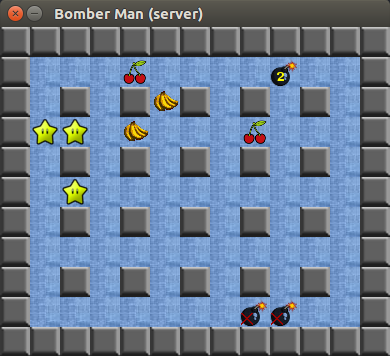
\includegraphics[scale=0.8]{image_jeu.png}
    \end{center}

    \clearpage

    \tableofcontents
    \clearpage

    \section{Introduction au projet}
    Pour ce projet il nous est demandé d'implémenter une version multi-joueurs du jeu Bomber Man à l'aide d'un serveur centralisé qui maintiendra à jour l'état courant du jeu.
    Seuls les clients sont en charge de l'interaction avec l'utilisateur (clavier et affichage graphique).
    Chaque client dispose d'une copie du modèle, qu'il doit maintenir à jour à travers des échanges réseaux avec le serveur.
    Nous possédons déjà un jeu fonctionnel qui comporte 2 maps, une implémentation de fruits pour regagner de la vie, puis le posage de bombes.
    \begin{center}
        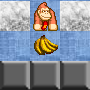
\includegraphics[scale=1]{fruit.png}
    \end{center}
    \begin{center}
        \caption{Fig 1.1 - Fruit en jeu}
    \end{center}
    \begin{center}
        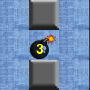
\includegraphics[scale=1]{post_break.png}
    \end{center}
    \begin{center}
        \caption{Fig 1.2 - Bombe en jeu}
    \end{center}
    Notre but est de trouver une solution pour réaliser ce qui a était dit jusqu'à présent.

    \section{Architecture et Implémentation}
    Pour répondre aux attentes du projet nous avons utilisé select (vu en cour) qui nous permet de savoir quand un client déjà présent ou non tente de modifier la grille ou de se connecter au serveur.
    Une fois que nous savons quel client essaye de nous contacter, nous allons analysé sa demande:

    -Si c'est la première fois qu'il se connecte nous allons l'inscrire dans notre table de clients avec son pseudo, attention il ne peut pas choisir un pseudo déjà utilisé actuellement ou dans le passé (depuis le dernier reboot du serveur).

    -Sinon nous recevons de cœur joie ses données, si il ne nous envoie pas de donnée il est alors déconnecté et son personnage est sauvegardé dans notre dictionnaire pour qu'il puisse se reconnecter exactement là ou il a était déconnecté.
    Ou alors il tente de nous indiqué qu'il se déplace ou bien qu'il pose une bombe, alors notre serveur joue le coup sur son propre model et diffuse le déplacement du personnage en question aux autres clients pour qu'ils puissent eux aussi appliquer le coup (idem pour une bombe).

    Nous vous invitons à regarder \hyperref[code]{ici} notre algorithme en pseudo-code puisque ce n'est qu'un court résumé du fonctionnement de notre serveur.

    Coté client, lors de la première connexion, il demande une connexion au serveur, puis envoie son pseudo à celui-ci pour qu'il puisse l'inscrire dans le dictionnaires des joueurs, suite à cela le serveur renverra la map, les joueurs, toutes les données nécessaire pour débuter une partie.
    Viens ensuite les interactions entre le serveur et le client. Tout d'abord le client attends un envoie du serveur avec un set.blocking(0) ce qui nous permet de réaliser des actions uniquement lorsque c'est nécessaire. Si joueur à fait une action, le serveur renverra une liste de deux cases avec en première position, une chaîne de caractère débutant par un "#" pour indiqué une action, suivis des données nécessaires pour appliquer l'action.

    Nous vous invitons à regarder \hyperref[code]{ici} pour plus de détails concernant les envoies du serveur au client.
    \clearpage
    \section{Vue d'ensemble fonctionnelle}
        \subsection{Fonctionnalités}
        Notre projet remplie toutes les conditions demandées, cela signifie qu'il est capable d'ajouter et de connecter plusieurs joueurs.

        \begin{center}
            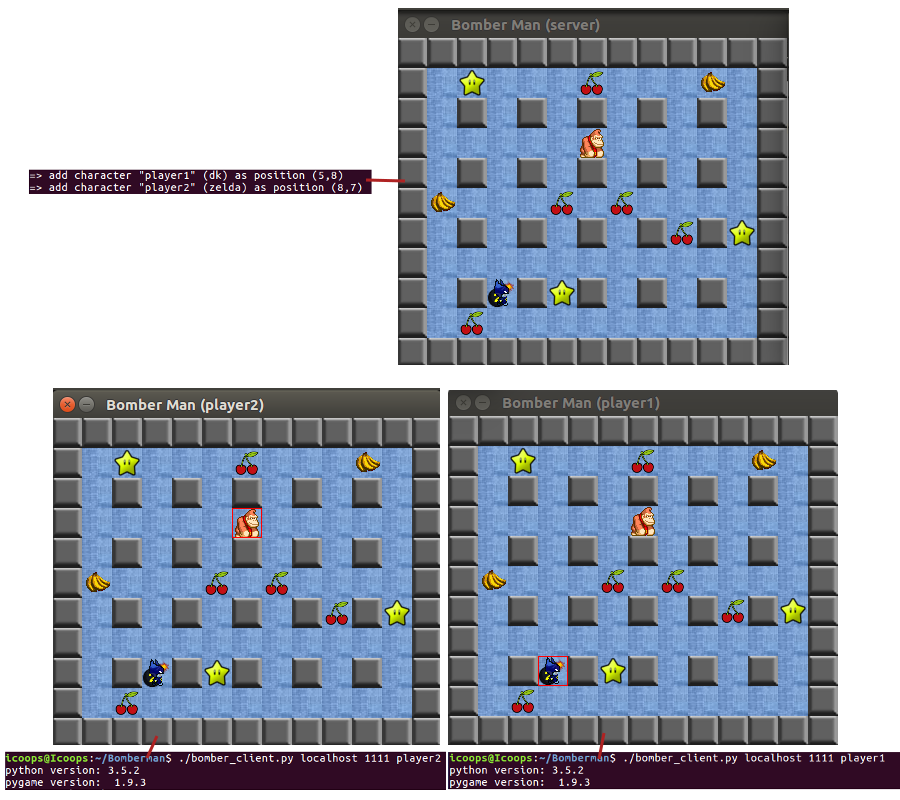
\includegraphics[scale=0.5]{connection.png}
        \end{center}
        \begin{center}
            \caption{Fig 3.1 - Déroulement d'une connexion}
        \end{center}
        \begin{center}
            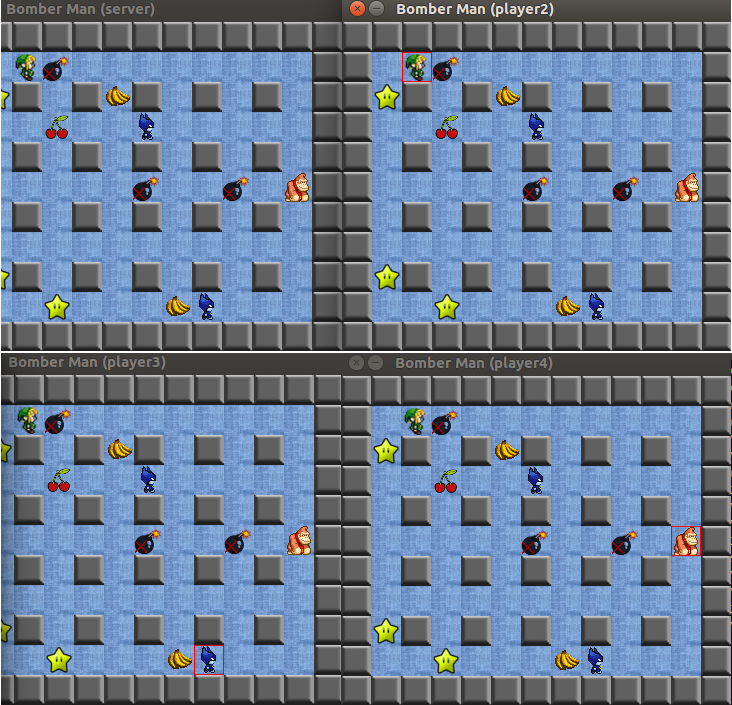
\includegraphics[scale=0.5]{4players.png}
        \end{center}
        \begin{center}
            \caption{Fig 3.2 - Connexion à 4 joueurs}
        \end{center}

        La partie réseau est aussi fonctionnelle, les joueurs sont capable de se déplacer sans problèmes, à chaque mouvement d'un joueur le serveur renvoie aux autres clients le personnage en question avec l'action "#move".

        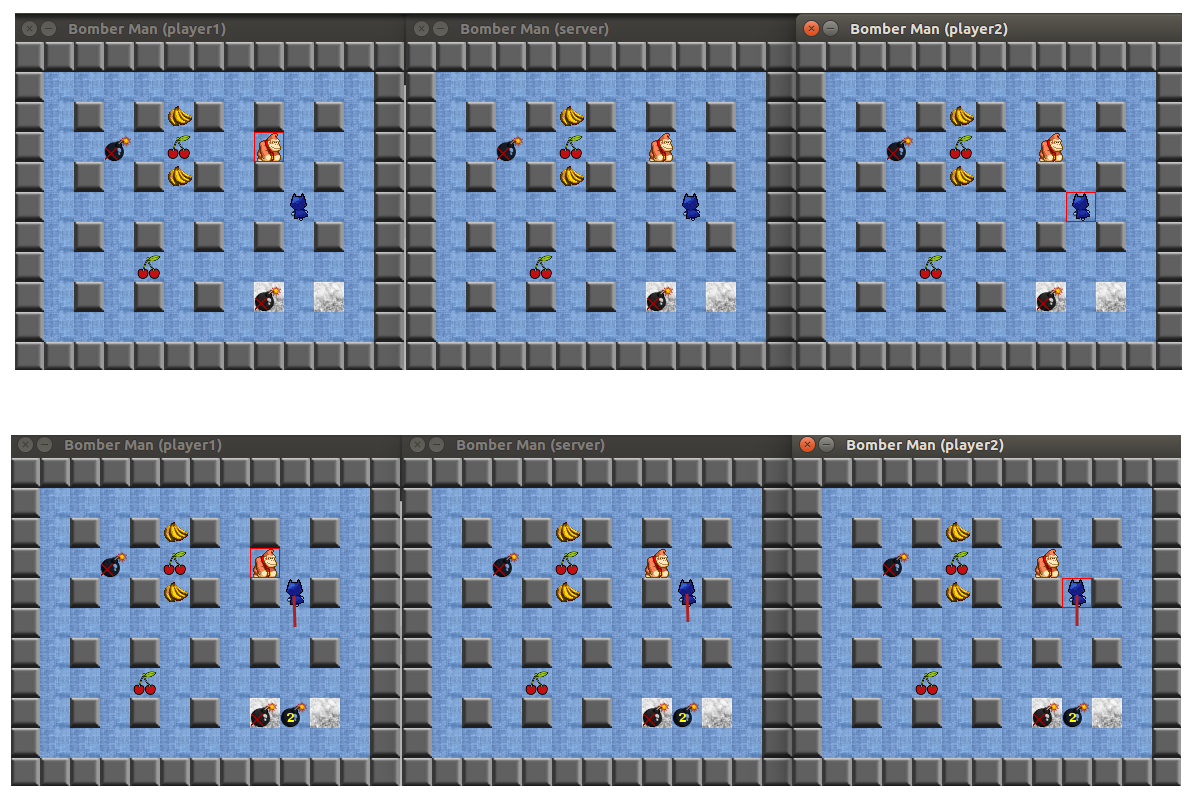
\includegraphics[scale=0.3]{deplacement.png}
        \begin{center}
            \caption{Fig 3.3 - Déplacement d'un joueur en ligne}
        \end{center}

        Pour ce qui est des bombes à chaque fois qu'un joueur pose un bombe sur la grille, le serveur le renvoie immédiatement aux autres pour qu'ils puissent être à jour, ce qui implique que chaque client à une explosion exactement au même moment.

        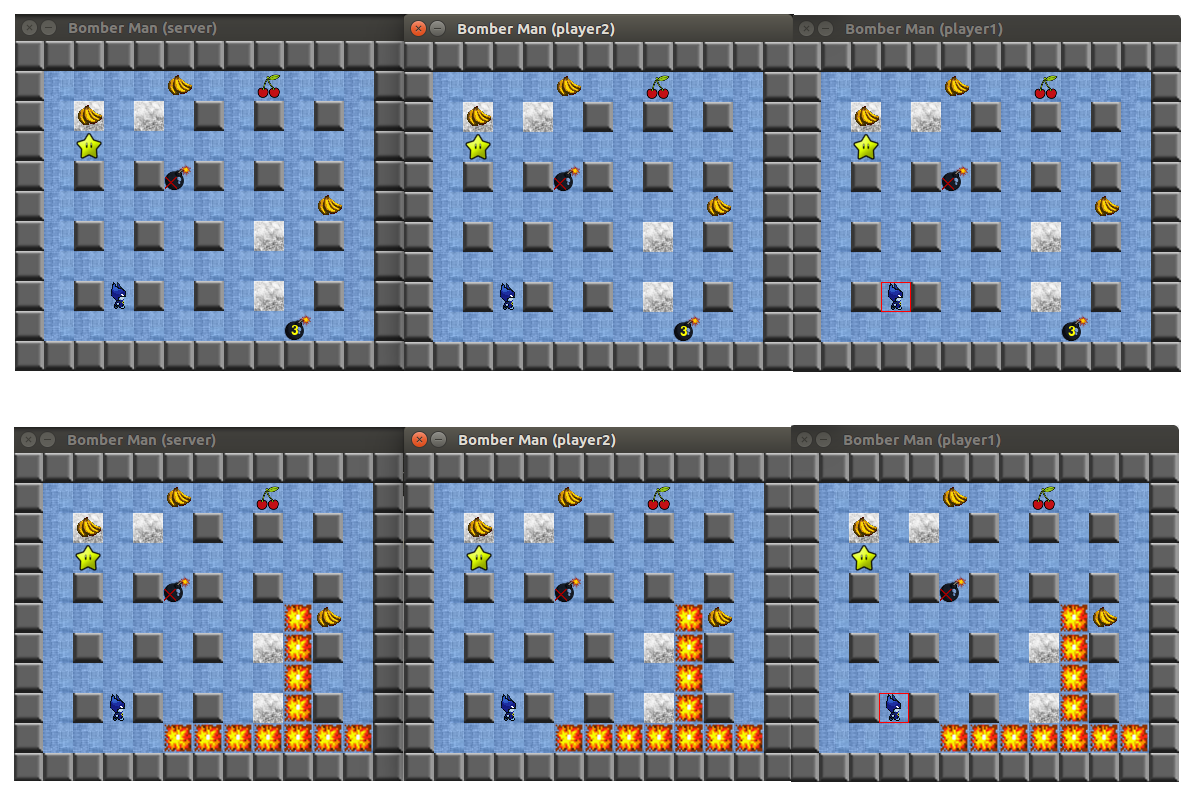
\includegraphics[scale=0.3]{explosion.png}
        \begin{center}
            \caption{Fig 3.4 - Explosion d'une bombe posé par un joueur en ligne}
        \end{center}

        Si une erreur survient soit par le serveur, tous les joueurs se verront déconnecter avec un message d'erreur.

        \begin{center}
            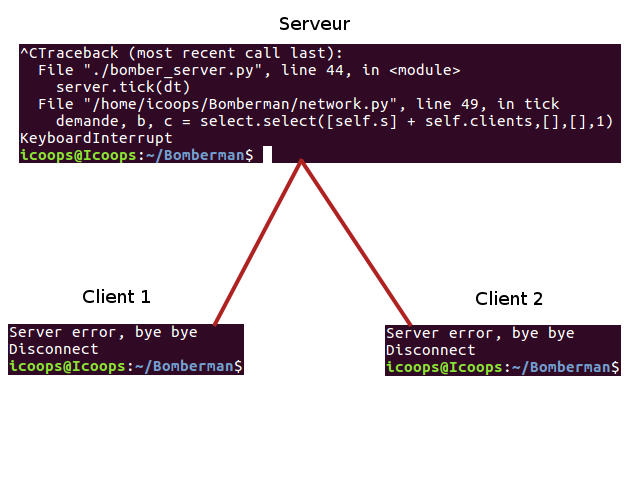
\includegraphics[scale=0.5]{deco_server.png}
        \end{center}
        \begin{center}
            \caption{Fig 3.5 - Déconnexion}
        \end{center}

        Et enfin si une personne est amené à mourir suite à une bombe alors ce personnage est tué sans être déconnecter puisqu’il pourra voir le déroulement de la partie des autres joueurs, c'est un mode spectateur.
        \begin{center}
            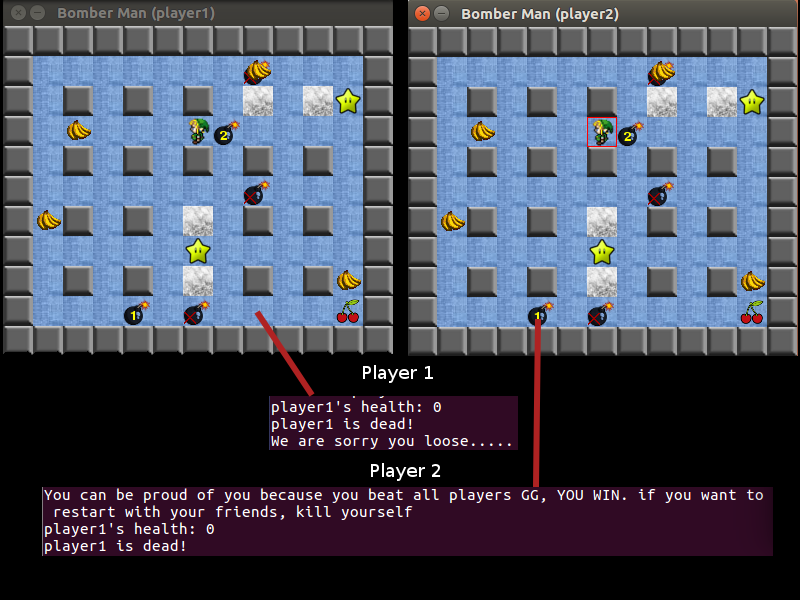
\includegraphics[scale=0.5]{mort.png}
        \end{center}
        \begin{center}
            \caption{Fig 3.6 - Mort d'un personnage en ligne}
        \end{center}

        \subsection{Bonus réalisés}
            \subsubsection{Incluant du réseau}
            Nous avons réalisé différents bonus incluant du réseau comme par exemple la sauvegarde de donnée par le pseudo. Nous avons dû créer un dictionnaire associant le personnage au pseudo,
            si un client avec un certain pseudo se déconnecte, alors nous sauvegardons toutes les données de son personnage que nous associons à son pseudo grâce à notre dictionnaire, et lors d'une connexion nous vérifions si le pseudo est inclut dans notre dictionnaire et si oui nous lui envoyons ses données à lui ainsi qu'aux autres avec l'instruction "#add" qui signifie ajouter un joueur.

            Ensuite nous avons développer la possibilité de recommencer une partie lorsque celle-ci est fini, c'est-à-dire que si il reste seulement un joueur de connecté à la suite d'un mort alors le serveur envoie un message à la dernière personne vivante lui indiquant que si il le souhaite il peut recommencer en se tuant. Pour réaliser cette fonctionnalité, nous avons dû crée une action supplémentaire qui se prénomme "#die", elle est envoyé à chaque mort d'un joueur au serveur par le client concerné. Le serveur cherche à savoir si il ne reste qu'un seul joueur si oui, alors il lui envoie un message.

            Puis enfin, les bombes aléatoire qui vont apparaître sur la carte toutes les 10 secondes. Pour ce faire nous avons un compteur qui toutes les 10 secondes demandes aux client d'ajouter une bombe en envoyant ces coordonnés.

            Notre projet est aussi capable de gérer plusieurs utilisateurs sans erreurs. (Plus de 2 joueurs)
            Pour finir, le serveur est capable d'envoyer au gagnant un message pour le féliciter de sa victoire.

            \subsubsection{Autres}
            Nous avons aussi crée d'autres bonus pour notre plaisir même si nous savons qu'il ne sauront pas noté nous tenions à les implémenter. Il existe deux nouveaux items, comme les étoiles qui rendent invincible une personne pendant un court temps et un item qui désactive les bombes pendant un court moment.
            \begin{center}
                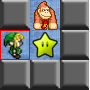
\includegraphics[scale=1]{etoile.png}
                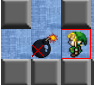
\includegraphics[scale=1]{disarm.png}
            \end{center}
            \begin{center}
                \caption{Fig 3.7 - Étoile}
                \caption{Fig 3.8- Anti-bombe}
            \end{center}
            Puis nous avons ajouté un effet aux bombes qui est de détruire des murs, nous avons alors crée une nouvelle image pour les murs qui ont était cassés.
            \begin{center}
                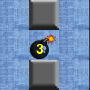
\includegraphics[scale=1]{post_break.png}
                
\includegraphics[scale=1]{break.png}
            \end{center}
            \begin{center}
                \caption{Fig 3.9 - Bombe devant des murs}
                \caption{Fig 3.10- Murs cassés par une bombe}
            \end{center}

        \subsection{Les problèmes}
        Nous avons réussi à localiser un problème qui est due à la pose de la bombe aléatoire, puisqu'il se peut qu'elle ait un court retard sur le serveur ce qui provoque alors la mort d'un personnage sur le serveur mais pas sur le client, cependant pour réalisé ce bug il faut avoir très peu de chance puisque les explosions sont décalés de quelques millièmes de secondes.

        \subsection{Améliorations proposées}
        Nous aurions pu améliorer notre systèmes de sauvegarde de donnés par un système de mot de passe qui serait donnée en paramètre lorsque l'on lance le programme et récupéré par le serveur avec une liste de liste.
        Enfin corriger le bug de la bombe qui se pause quelques millième de seconde trop tôt.

    \clearpage
    \section{Bilan du projet}

    Pour résumé nous avons implémenté le multijoueur ainsi que différents bonus comme la destruction de mur, une nouvelle map, de nouveaux "items", un système de sauvegarde de donné grâce au pseudo, la possibilité de recommencer une partie et la pose de bombe aléatoire toutes les 10 secondes.
    Nous avons beaucoup appris sur la conception d'un jeu multijoueur puisque c'est la première fois que nous utilisons des sockets. Nous pourrons utilisé ces compétences acquises pour nos propres projets personnels.
    Pour finir, nous avons trouvé que le projet était en parfaite harmonie avec les cours donnés et la liberté du projet, ce qui nous a permis de concevoir ce que l'on souhaite, même si nous avons eu quelques difficultés les cours ont pu nous permettre de franchir des caps et ainsi en apprendre d'avantage.

    \clearpage
    \nocite{*}
    \bibliographystyle{plain}
    \bibliography{biblio}

    \label{code}
    \begin{verbatim}
COTE SERVEUR:
clients = []

Function tick_network(clock):
    On vérifie s'il faut poser une bombe:
        Si oui, on pose une bombe et on envoie une action "#bomb" aux clients.
    demande,x,y = select.select(socket + clients,[],[],1)
    For client in demande:
        Si le client demande une connexion:
            On accepte
            Ajout du client dans un champ de clients
        Sinon:
            On récupère les données
            On décode les données
            commands = Split de la data (pour enlever les espaces dans data)
            Si pas de donnée:
                char = personnage du joueur
                On vérifie si le pseudo est déjà sauvegardé
                    account = ajout de [pseudo, client, personnage]
                On demande aux clients de supprimer le personnage.
                On supprime le client de la liste clients
                On supprime son pseudo du dictionnaire de pseudo.
            Si commands[0] == "#nickname":
                On vérifie si le personnage existe
                Si il n’existe pas:
                    On regarde s'il est inscrit dans account.
                        Si oui, on envoie la demande d'ajout aux autres clients.
                Si il n'était pas dans les clients:
                    On ajoute le personnage
                    On ajoute son pseudo dans le dictionnaire des pseudo
                    On envoie la demande d'ajout aux autres clients.
                Sinon:
                    On ferme le clients.
            Si (commands[0] == "#die"):
                On supprime le personnage (au cas où, sans erreur)
                Si il n'y a plus de personnage:
                    On rajoute les joueurs sur la grille grâce au dictionnaire
                    de pseudo.
                    On initialise la map, les fruits, les bombes.
                    Ajout de 10 fruits.
                    On envoie une commande "#rematch" aux clients, avec la map.
                Si il ne reste plus qu'un joueur:
                    On envoie une commande "#winner" au client.
            Si (command[0] == "#move"):
                On envoie une action "#move" avec les personnages et les bombes
            Si (commands[0] == "#bomb"):
                On envoie les bombes aux joueur avec l'action "#bomb"

COTE CLIENT:
__init__(host, port, nickname):
    Initialisation host,port,socket.
    Envoie de l'action "#nickname" au serveur.
    On attend de recevoir des données.
    Si pas de donnée:
        Fermeture de la socket.
    Sinon:
        On charge les données dans la map du client

Fonction tick_client(clock):
    On attends les données
    On essaye de recevoir les données.
    Si pas de donnée:
        Print("serveur erreur")
        return False
    Sinon:
        Si donnée[0] = "#bomb":
            On charge les bombes avec le deuxième argument.
        Si donnée[0] = "#move":
            On charge les bombes et le personnage.
        Si donnée[0] = "#add" ou "#del" ou "#rematch":
            On met à jour les joueurs.
        Si donnée[0] = "#rematch":
            Mise à jour de la map, des fruits, des bombes.
        Si donnée[0] = "#winner"
            Affichage du message.
        Si donnée[0] = "#add_bomb"
            Le client pose lui même une bombe avec des paramètres particuliers.
        For personnage dans les personnages:
            Si nom du personnage = Pseudo
                ajout dans le model du personnage dans le champ joueur.
    \end{verbatim}

\end{document}
